%!TEX root = ../main.tex
\chapter{Validation of the time calibration}
\label{chap:TimingValidation}

It is necessary to perform a validation of the timing calibration (see chapter \ref{chap:TimingCalib}). The recorded electron data is used because electromagnetic showers are quasi-instantaneous and thus are perfect to validate the time calibration. The electron dataset used in this study is selected based on criteria described in section \ref{subsec:elec_sel}. The same calibration constants and correction constants determined from the muon data are applied to the electron data.

\section{Time of the first hit for electrons}

The time of the first hit for 20 GeV electrons after the timing calibration with the calibration constants obtained from the muon data is shown in figure \ref{fig:Timing_electrons}. In addition, the distribution is compared to the time distribution from the muon data. It is expected to obtain a similar or better time resolution for electrons compared to muons.

The peak of the electron time distribution in figure \ref{fig:Timing_electrons} is shifted to the left by around 10 ns. This time offset is expected due to a change in the trigger configuration (see section \ref{sec:TBsetup}). This offset is consistent with the difference between the trigger configurations in cable length to route the trigger signal.

However, the time distribution of electrons presents a large tail to the right and is much wider than the one for muons. This is not expected first and this could be related to the number of hits which is much higher in an electromagnetic shower than from a muon and as well that the deposited energy in a single cell can be over 100 MIPs (see figure \ref{fig:eHitVal}).

\begin{figure}[htbp!]
	\centering
	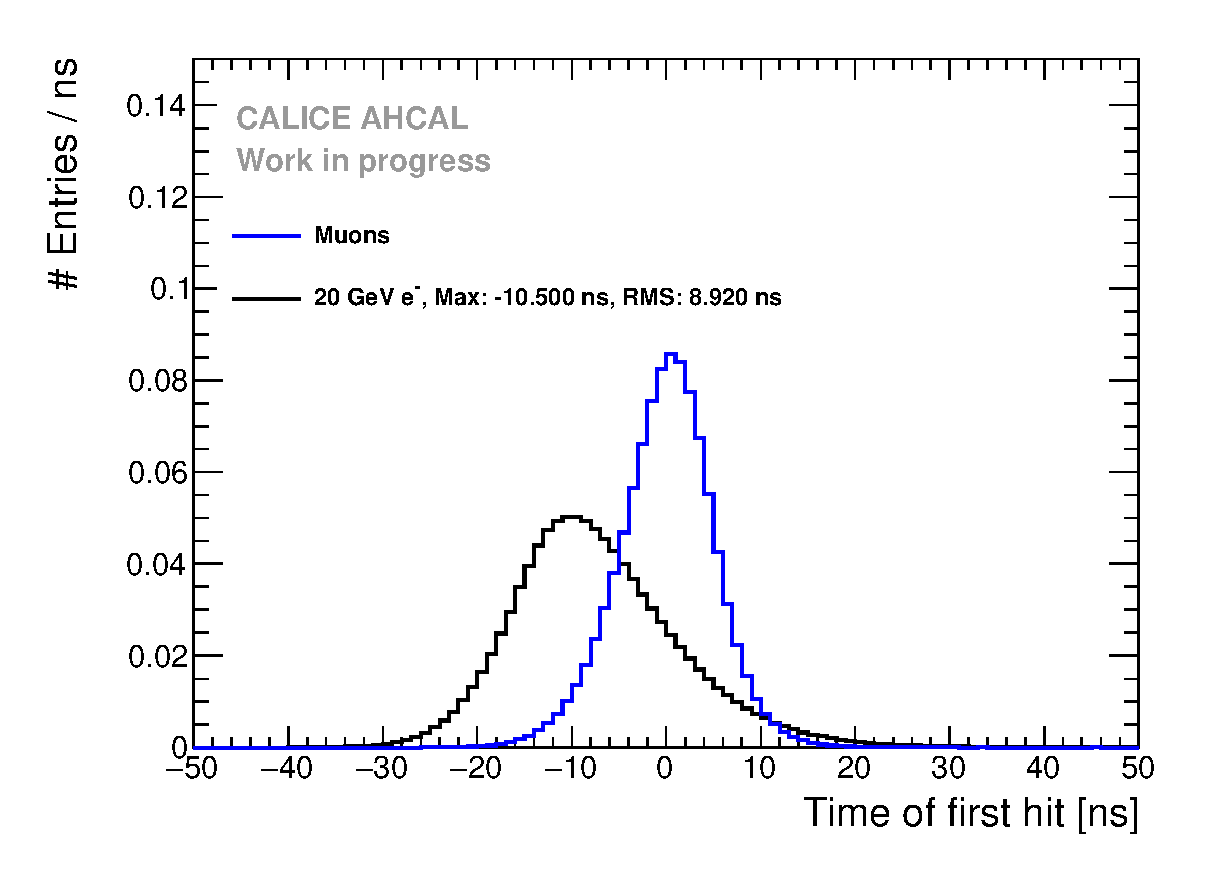
\includegraphics[width=0.6\textwidth]{../Thesis_Plots/Timing/Electrons/Plots/Timing_AllLayers_AfterMuons.eps}
	\caption{Time of the first hit distribution for 20 GeV electrons after applying the calibration constants extracted from the muon data. The blue distribution represents the time of first hit distribution obtained with muons.}
	\label{fig:Timing_electrons}
\end{figure}

\section{Effect of the number of triggered channels on the time distribution}
\label{subsec:ped_shift}

For the energy measurement, there is a known and well understood feature of the SPIROC chip \cite{Hartbrich2012}, that induces a shift in the baseline of the ADC signal for large pre-amplifier loads, i.e. for large charges on the SPIROC input channels. This feature may be also present for the timing measurement. Since it is a priori not clear if the effect depends on the number of triggered channels \textit{in a chip} or the energy sum \textit{in a chip}, the time correction has been checked using both variables. It turned out that the time correction as a function of the number of triggered channels over 0.5 MIP in a chip gives better results than the time correction as a function of the energy sum in a chip. This is not totally understood why.

The mean time of first hit as a function of the number of triggered channels over 0.5 MIP in a chip is shown in figure \ref{fig:nhits_profile}. A time shift up to 20-40 ns can be seen depending on the number of triggered channels in a chip. The cause of the observed effect is most likely due to an element in the chip called a \textit{delay box} that gets unstable with a high charge going through the chip. This chip element is responsible for the hold signal of the TDC ramp in the chip. The hold signal is delayed, and thus a higher TDC ramp value than the one expected is sampled.

\begin{figure}[htbp!]
	\begin{subfigure}[t]{0.49\textwidth}
		\centering
		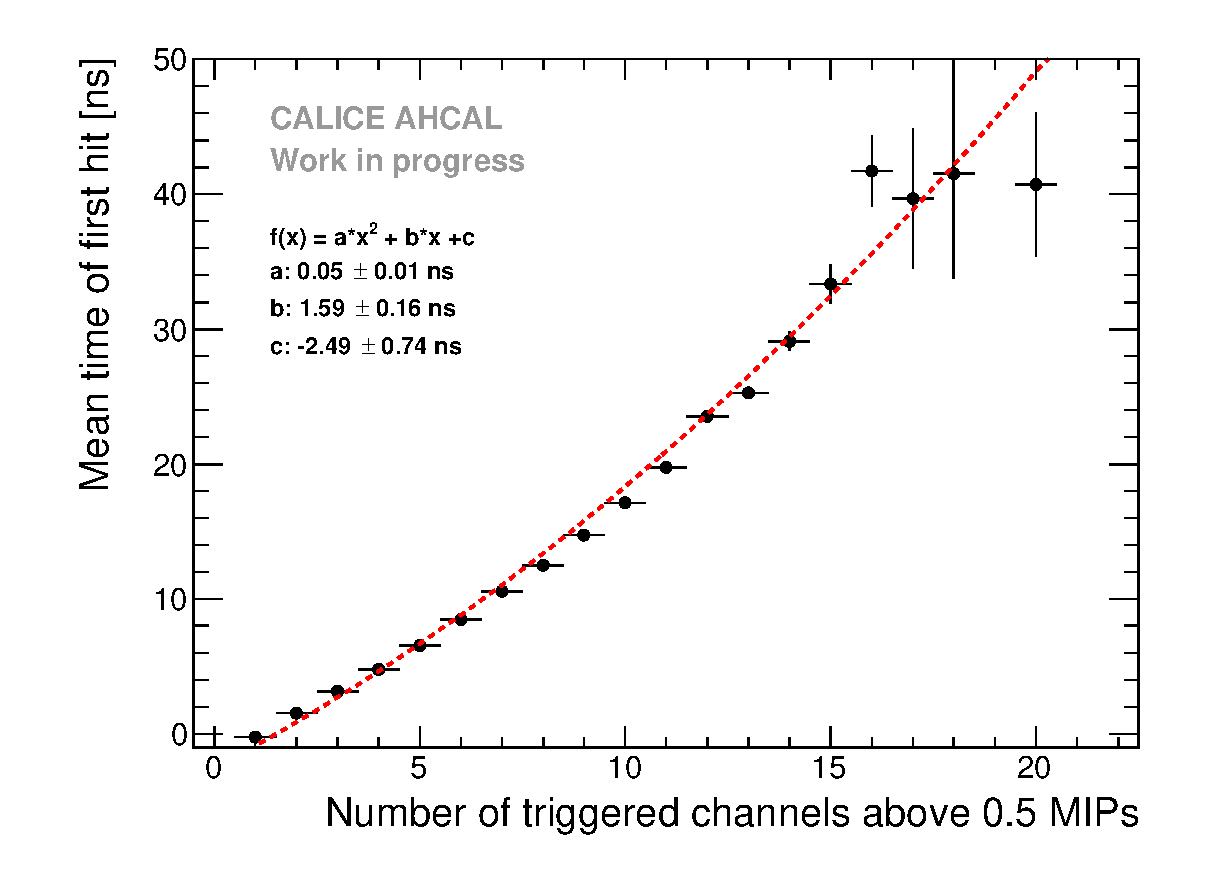
\includegraphics[width=1\textwidth]{../Thesis_Plots/Timing/Electrons/Plots/NumberHits_Dependance_AllEnergies.eps}
		\caption{}\label{fig:nhits_profile}
	\end{subfigure}
	\hfill
	\begin{subfigure}[t]{0.49\textwidth}
		\centering
		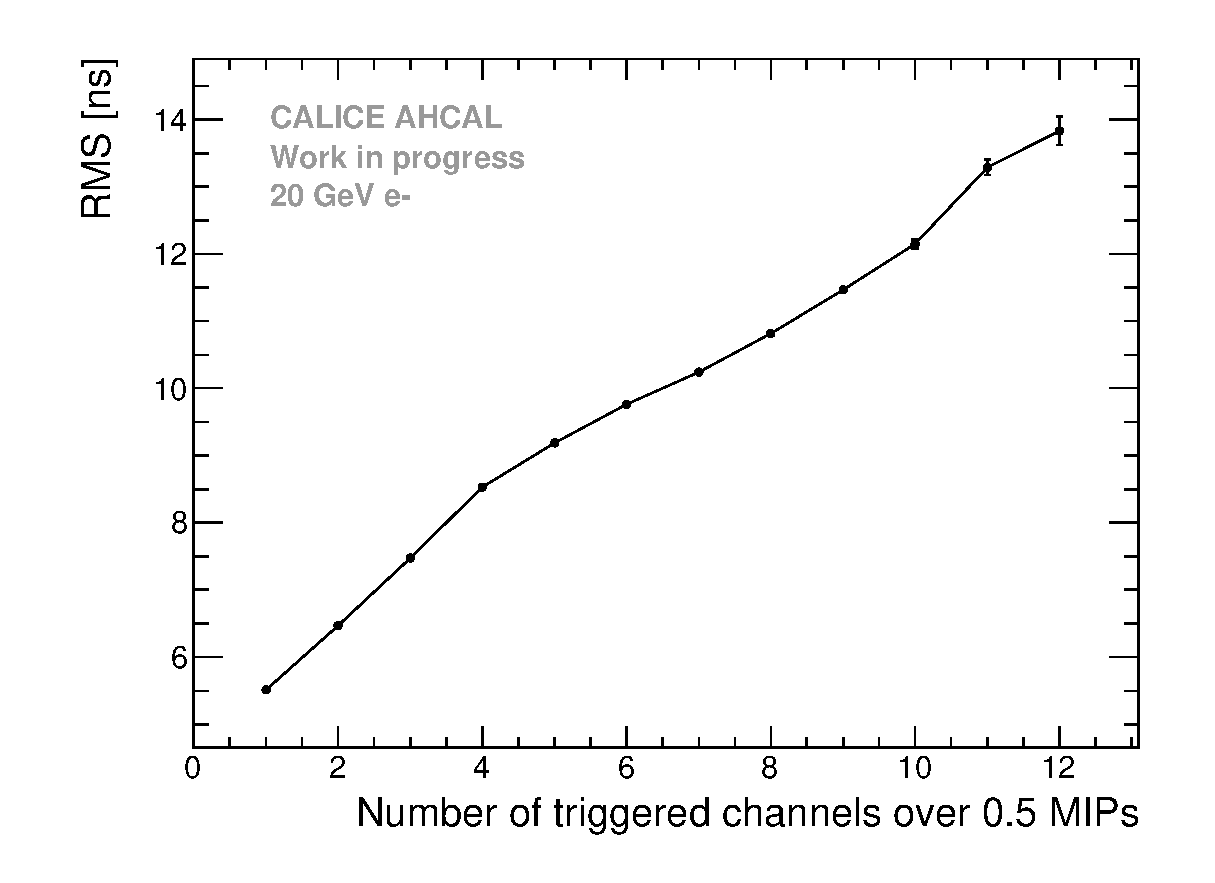
\includegraphics[width=1\textwidth]{../Thesis_Plots/Timing/Electrons/Plots/ParametrisationPedestalShift_20GeV.eps}
		\caption{}\label{fig:RMS_nHits}
	\end{subfigure}
	\caption{\subref{fig:nhits_profile}) Mean time of the first hit as a function of the number of triggered channels above 0.5 MIP in a chip. The mean time shifts upwards with the increase of triggered channels leading to large tails in the time distribution. A second order polynomial fit is done for the time correction shown by the red dashed line. \subref{fig:RMS_nHits}) The RMS of the time of first hit distribution as a function of the number of triggered channels above 0.5 MIP in a chip for 20 GeV electrons. The RMS of the time distribution can increase up to 10-15 ns for a high number of triggered channels in a chip.}
\end{figure}

The time correction parameters are determined by a $2^{nd}$ order polynomial fit to the data as shown by the red line in the figure \ref{fig:nhits_profile}. In order to determine a reliable time correction, the time correction parameters are determined combining all the electron data. A priori, this effect should not be dependent on the beam energy. However, a dependence is seen (see section \ref{subsec:Systematic_Correction}) and shows that the effect is not totally understood. Therefore, the differences are treated as systematic uncertainty. This effect may be chip-dependent and the parameters for the correction may differ from chip to chip. However, the limited amount of data does not allow to determine a correction function for each chip. Therefore, a global function is used to correct the time in the data.

Figure \ref{fig:Nhit_residuals} shows the residuals of the mean time of first hit as a function of the number of triggered channels above 0.5 MIP in a chip ($N_{trig/chip}$) after the correction. The correction has been applied to all electron samples separately in order to evaluate the systematic uncertainty of the correction. Three ranges in $N_{trig/chip}$ have been defined delimited by the red lines to estimate the uncertainty. To not overestimate the uncertainty, half of the residual envelope is taken as uncertainty. For 0 < $N_{trig/chip}$ < 5, a systematic uncertainty of 2 ns is taken, For 5 $\leq$ $N_{trig/chip}$ < 12, a systematic uncertainty of 5 ns is taken and finally for $N_{trig/chip}$ $\geq$ 12, a systematic of 7 ns is taken. Finally, the uncertainty for the mean time of the first hit is computed \textit{for each bin of energy and radius} by weighting according to the fraction of hits in each of the three regions following equation \ref{eq:syst_nHits}. As the uncertainties in the three ranges are correlated, a conservative way is to add linearly the uncertainties.

\begin{equation}
  \sigma = n_1 \times \sigma_1 + n_2 \times \sigma_2 + n_3 \times \sigma_3 \label{eq:syst_nHits}
\end{equation}

with $\sigma_1$ = 2 ns, $\sigma_2$ = 5 ns, $\sigma_3$ = 7 ns, $n_1$ the fraction of hits for the i-th bin in the region 0 < $N_{trig/chip}$ < 5, $n_2$ the fraction of hits for the i-th bin in the region 5 $\leq$ $N_{trig/chip}$ < 12 and $n_2$ the fraction of hits for the i-th bin in the region $N_{trig/chip}$ $\geq$ 12 and such as $n_1 + n_2 + n_3$ is equal to one in the i-th bin.

\begin{figure}[htbp!]
  \centering
  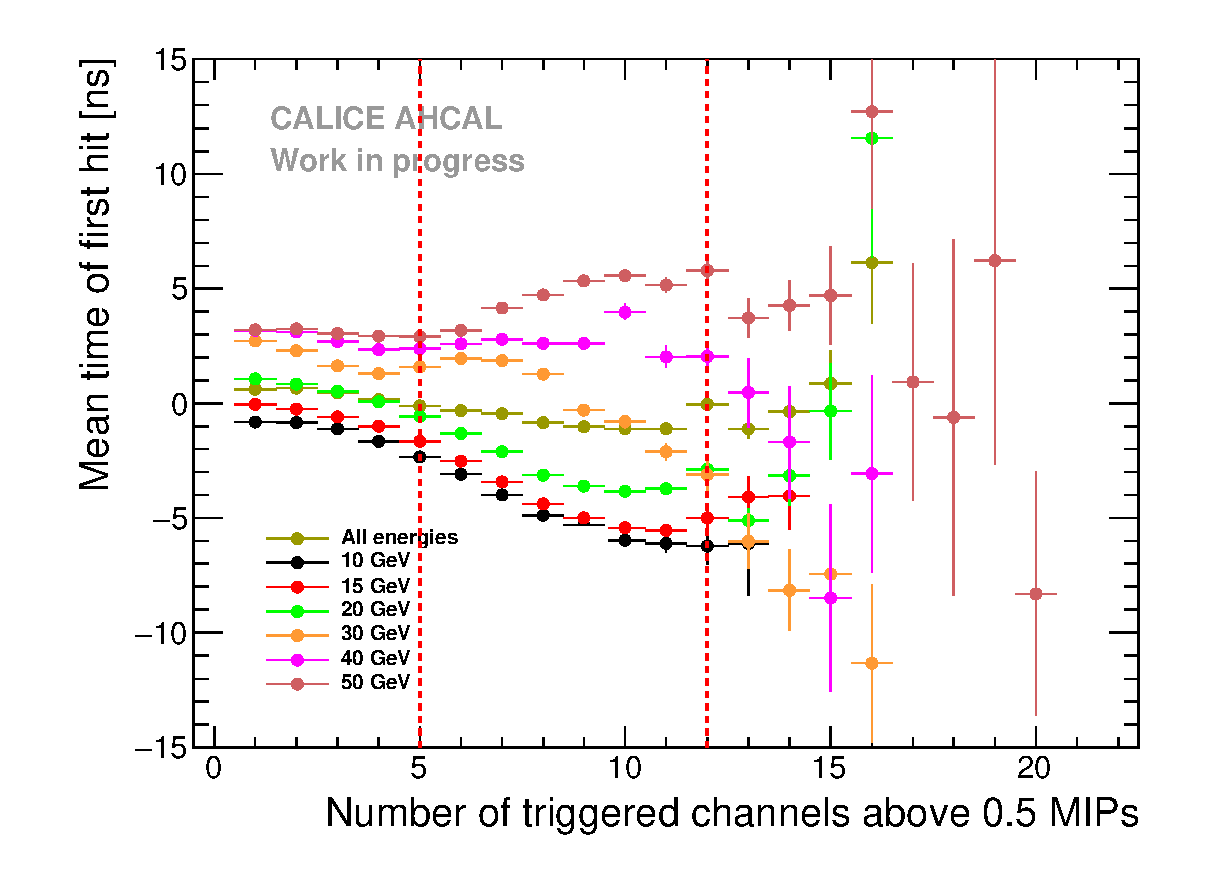
\includegraphics[width=0.6\textwidth]{../Thesis_Plots/Timing/Electrons/Plots/CheckCorrection.eps}
  \caption{Residuals of the mean time of the first hit as a function of the number of triggered channels above 0.5 MIP in a chip after correction. The correction has been applied to all electron samples separately to evaluate the systematic uncertainty. The vertical red lines delimit the three sections used for the systematic uncertainty.}
  \label{fig:Nhit_residuals}
\end{figure}

The figure \ref{fig:RMS_nHits} shows the RMS of the time distribution increasing with the number of triggered channels over 0.5 MIP in a chip. As expected, if a single channel in a chip triggers, the RMS of the time distribution ($\sim$ 5.5 ns) is close to the time resolution for muons as shown in figure \ref{fig:RMS_nHits}.

The time resolution (RMS) of the AHCAL is expected to be slightly dependent on the electron beam profile that affects directly the number of triggered channels in a chip. In addition, as the time resolution (RMS) of the AHCAL is dependent on the number of triggered channels in a chip, i.e the number of hits in the calorimeter, it is expected that the time resolution increases as a function of the electron beam energy as the number of hits in a EM shower is proportional to its energy.

\section{Time of the first hit after correction}
\label{subsec:Electron_Final}

The distribution of the time of the first hit for 20 GeV electrons is shown in figure \ref{fig:timing_electrons_corr} before and after the time correction as a function of the number of triggered channels in a chip. The correction improves the RMS of the distribution by around 10\%, as well as the distribution appears more Gaussian-like.

However, there is still a discrepancy of around 54.6\% from the time resolution obtained from muons (see section \ref{subsec:Muon_final}). This is because the RMS of the time distribution increases as a function of the number of triggered channels in a chip (see figure \ref{fig:RMS_nHits}). The increase of the RMS can't be corrected unlike the mean of the time distribution.

The increase of the width of the time distribution is parametrized from data for the simulation. More details about the parametrization implementation in the simulation are given in the appendix \ref{appendix:ped_shift}.

\begin{figure}[htbp!]
	\begin{subfigure}[t]{0.49\textwidth}
		\centering
		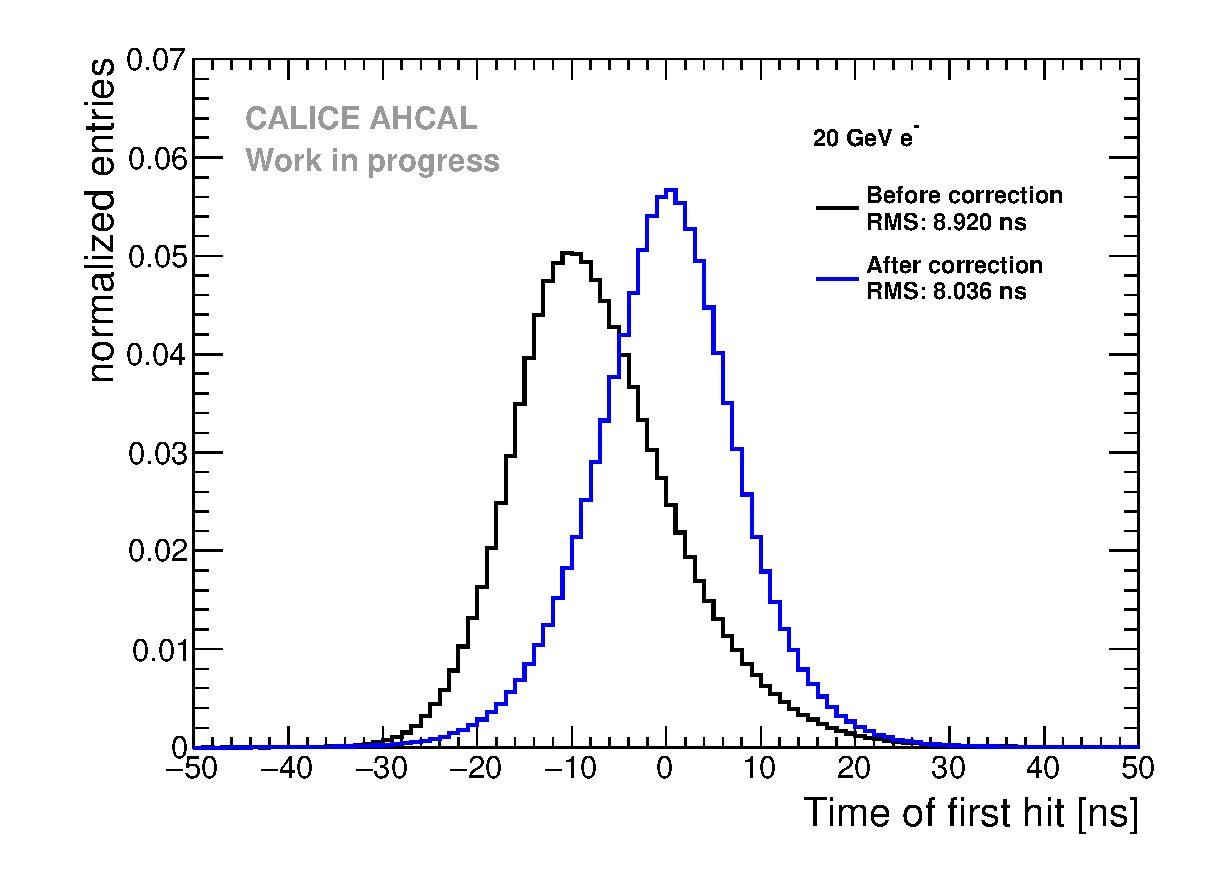
\includegraphics[width=1\textwidth]{../Thesis_Plots/Timing/Electrons/Plots/Timing_AllLayers_20GeV.eps}
		\caption{}\label{fig:timing_electrons_corr}
	\end{subfigure}
	\hfill
	\begin{subfigure}[t]{0.49\textwidth}
		\centering
		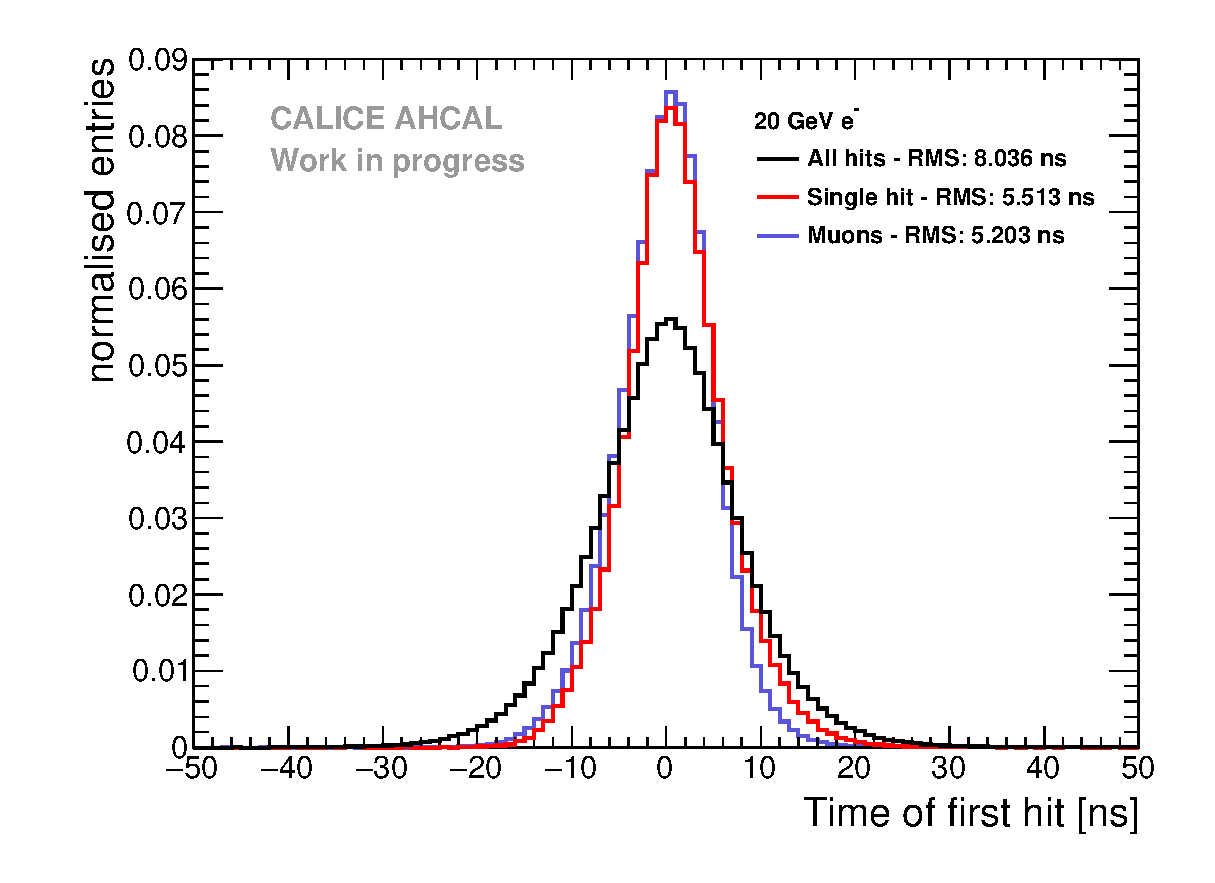
\includegraphics[width=1\textwidth]{../Thesis_Plots/Timing/Electrons/Plots/ComparisonAll_ElectronsSingleHit.eps}
		\caption{}\label{fig:timing_electron_muon_comp}
	\end{subfigure}
	\caption{\subref{fig:timing_electrons_corr}) Time of the first hit distribution for 20 GeV electrons after the number of triggered channel in a chip correction. \subref{fig:timing_electron_muon_comp}) Comparison of time distribution of 20 GeV electrons and muons. The electron time distribution is very similar to the muon time distribution when only a single channel triggers in a chip.}
\end{figure}

A comparison of the time distribution from electrons and from muons has been done in order to further cross-check the calibration (see figure \ref{fig:timing_electron_muon_comp}). The time resolution from electrons is very similar to the time resolution from muons when only a single channel triggers in a chip. The difference in time resolution is around 6\%.

All electron runs have been carefully checked to validate the timing calibration. The figure \ref{fig:all_electron_energies} shows the comparison of the time distribution from electrons between 10 GeV to 50 GeV beam energies. The mean of the time distributions is very similar. The RMS of the time distributions increases as expected and it varies between 7.94 ns at 10 GeV and 8.88 ns at 50 GeV corresponding to an increase of 11.8\%. A large deviation from the 20 GeV electron time distribution for energies above is visible after 20-30 ns. This may be due to slight differences in beam profile for each beam energy, the increase of the time resolution for higher beam energies and the time correction as a function of the number of triggered channels in a chip that is not perfect. However, within 3 sigmas, the time distributions differ up to 10-20\%. In addition, a similar effect is visible for negative times, thus different noise levels due to different beam rates might also play a role.

\begin{figure}[htbp!]
	\centering
	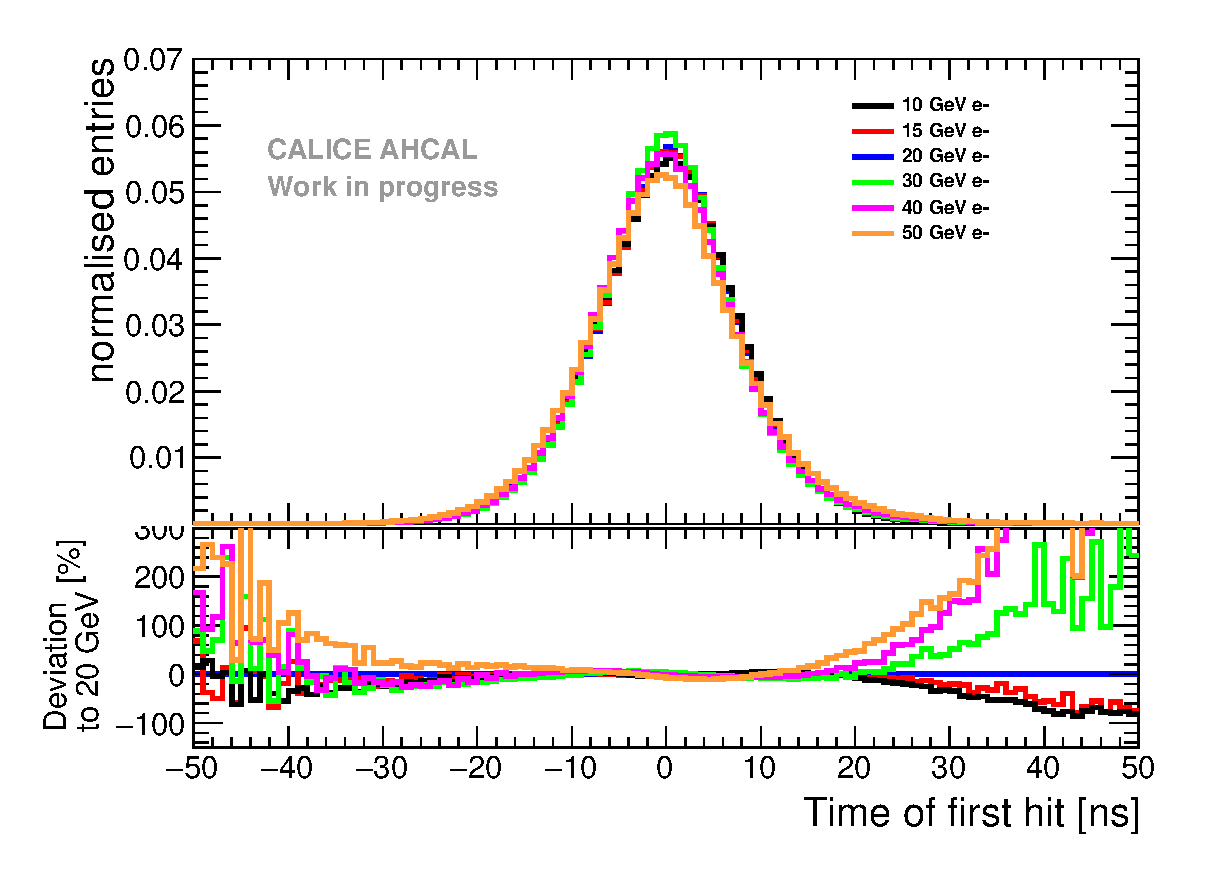
\includegraphics[width=0.6\textwidth]{../Thesis_Plots/Timing/Electrons/Plots/ComparisonDataEnergies.eps}
	\caption{Comparison of the time of first hit distribution for electron beam energies between 10 GeV and 50 GeV. The bottom plots shows the relative difference to the 20 GeV electron time distribution.}
	\label{fig:all_electron_energies}
\end{figure}

\section{Transportability of the calibration}

A check on the validity of the calibration for other data-taking periods has been performed on another dataset from a testbeam at DESY II in May 2016. The goal is to understand the transportability of the time calibration. The setup was composed of the same layers 11 to 14 used at CERN in July 2015. In order to have enough hits in all layers, an aluminum absorber of 3 $X_{0}$ was placed in front of the detector in a 3 GeV electron beam.

The same time calibration constants determined from the CERN muon and electron data were used, except that a re-calibration of the time reference triggers ($T_{0}$) and the trigger time offset was necessary. This is due to different setups in the cabling and trigger electronics. For this setup, only two $T_{0}$ channels on the layer 14 were working properly.

Figure \ref{fig:TBMay2016} shows the distribution of the time of first hits for layer 12 to 14, the layer 11 is ignored as the same behavior seen in the CERN dataset is also seen for this dataset, for all hits in black and for events with only single hits per chip in blue. The time distribution is compared to the time distribution for the layers 12 to 14 of 10 GeV electrons recorded at CERN in July 2015.

The time resolution is around 6.9 ns which is very slightly worse than ($\sim$ 6\% difference) the time resolution using the same layers at the CERN testbeam. This difference seen in time resolution can be related to the slightly worse (around 4\%) time reference resolution.

\begin{figure}[htbp!]
	\centering
	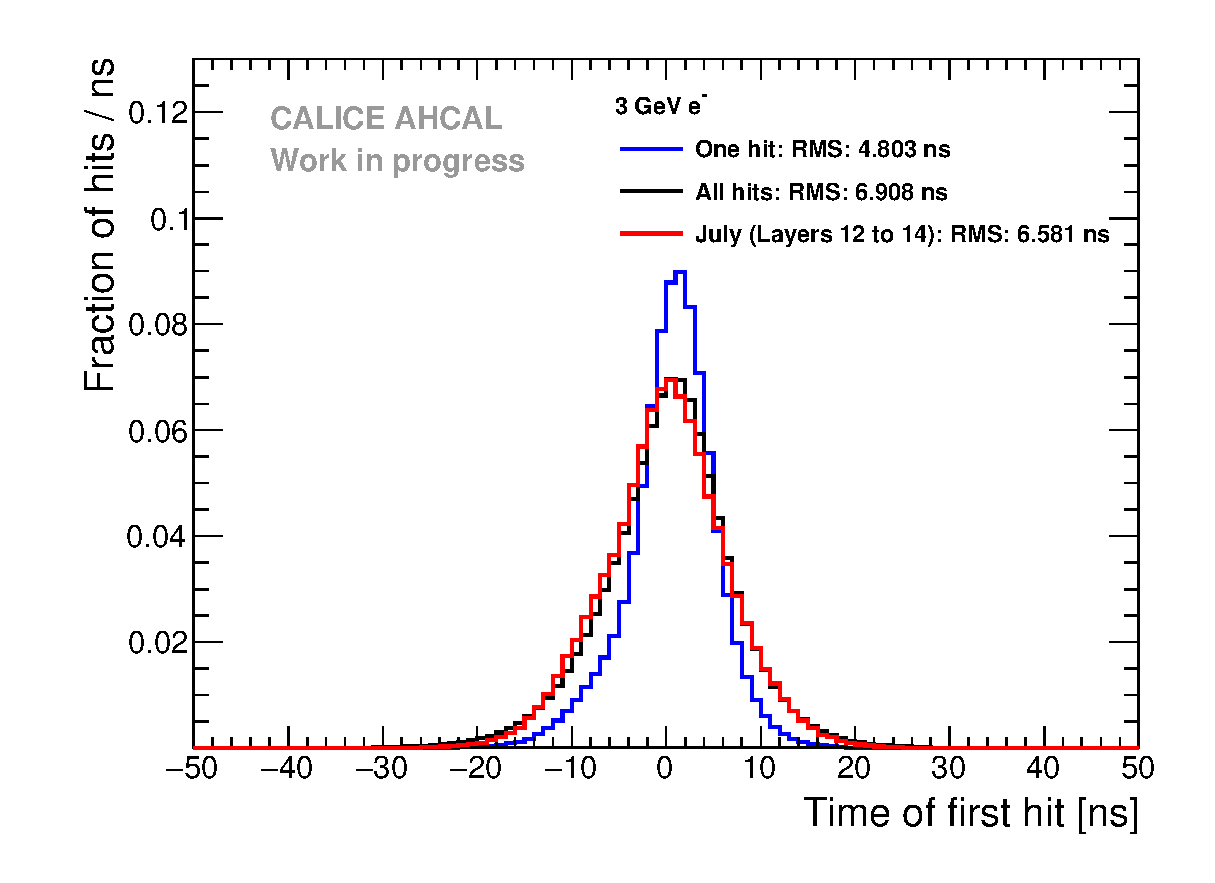
\includegraphics[width=0.6\textwidth]{../Thesis_Plots/Timing/Electrons/Plots/Timing_May2016_BigLayers.eps}
	\caption{Time of the first hit distribution for 3 GeV electron showers at the DESY II testbeam in May 2016 combining layers 12 to 14 in black. The blue distribution is the time of first hit in the case of events in which only single hits in a chip are taken. The red distribution is the time of first hit for the same layers in 10 GeV electrons collected at the CERN SPS in July 2015.}\label{fig:TBMay2016}
\end{figure}

We can learn from this study, that the time calibration constants determined in a specific dataset can also be used for another dataset \textit{with the same layers}. The timing calibration values depends mainly on hardware and not so much on the environment.

\section{Estimation of the systematic uncertainty of the time correction on the time of first hit distribution}
\label{subsec:Systematic_Correction}

A global correction is used for the time correction as a function of the number of triggered channels. A priori, it is not clear if the time correction is chip-dependent and it could not be verified. Therefore, a systematic uncertainty of the time correction on the time of first hit distribution needs to be estimated.

A study has been done to estimate this uncertainty by looking at the time distribution for events where the center of gravity of the shower is in one of the four center tiles of the detector. The four center tiles are chosen due to the higher event rate. This gives four different time distributions that can be compared and that can help to estimate the impact of the time correction as a function of the number of triggered channels in a chip in different sections of the detector. This has been performed for electron beam energies of 10 GeV and 50 GeV.

The figure \ref{fig:timing_syst_10GeV} and \ref{fig:timing_syst_50GeV} show the time distribution for events with the center of gravity in each one of the four tiles for 10 GeV and 50 GeV electron beam energies respectively. For both beam energies, the mean of the time distributions are very similar and are close to 0 ns. The RMS of the time distributions vary between 7.12 ns and 7.45 ns at 10 GeV and between 8.1 ns and 8.8 ns at 50 GeV. The mean deviation from the top left tile is shown in black line in the bottom plots. A relative deviation over 30\% to the top left tile can be seen in the region over 30 ns and under -30 ns. The mean deviation curve in figure \ref{fig:timing_syst_50GeV} is taken as a systematic uncertainty on the bin content in the data truncated in the region from -30 ns to 30 ns. Outside of this region, a systematic uncertainty of 50\% on the bin content is taken.

\begin{figure}[htbp!]
	\begin{subfigure}[t]{0.49\textwidth}
		\centering
		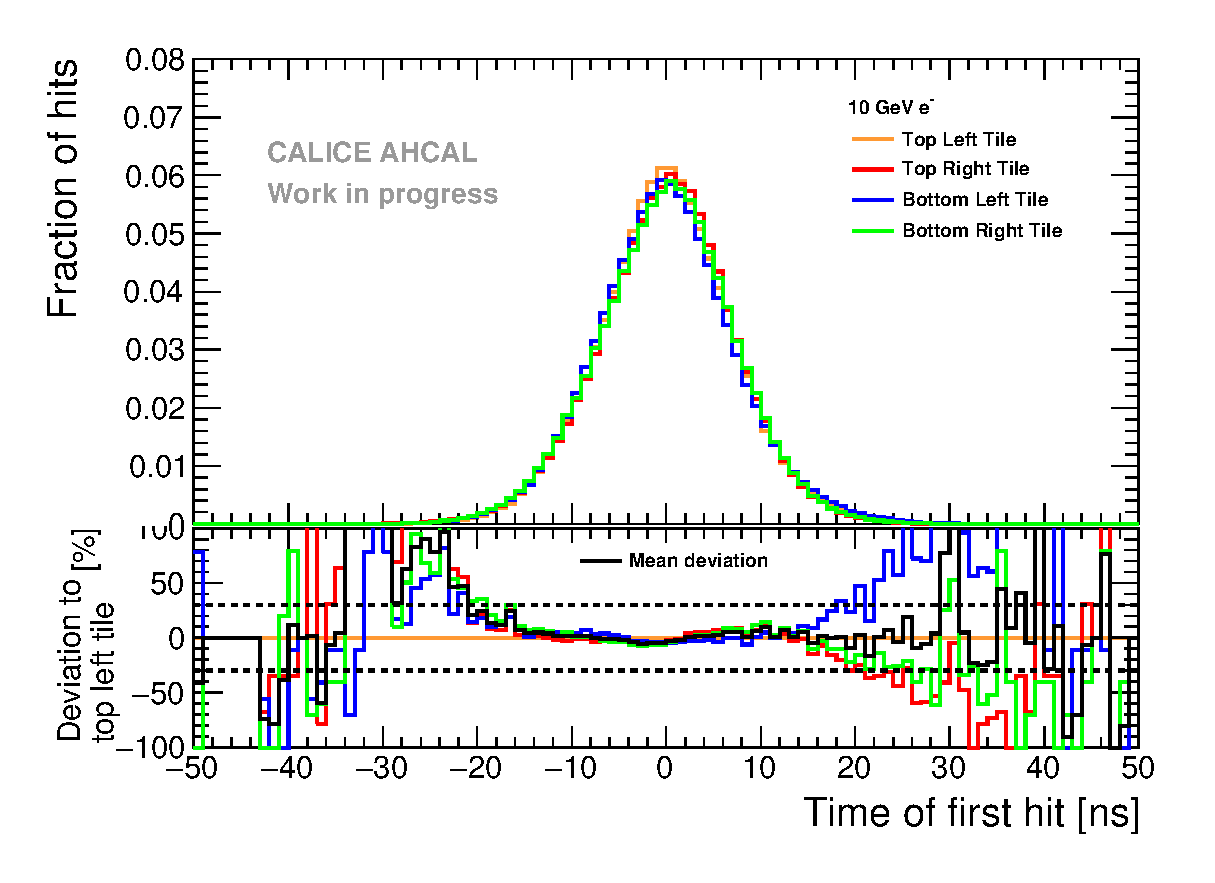
\includegraphics[width=1\textwidth]{../Thesis_Plots/Timing/Electrons/Plots/Systematic_Inhomogeneity_10GeV.eps}
		\caption{}\label{fig:timing_syst_10GeV}
	\end{subfigure}
	\hfill
	\begin{subfigure}[t]{0.49\textwidth}
		\centering
		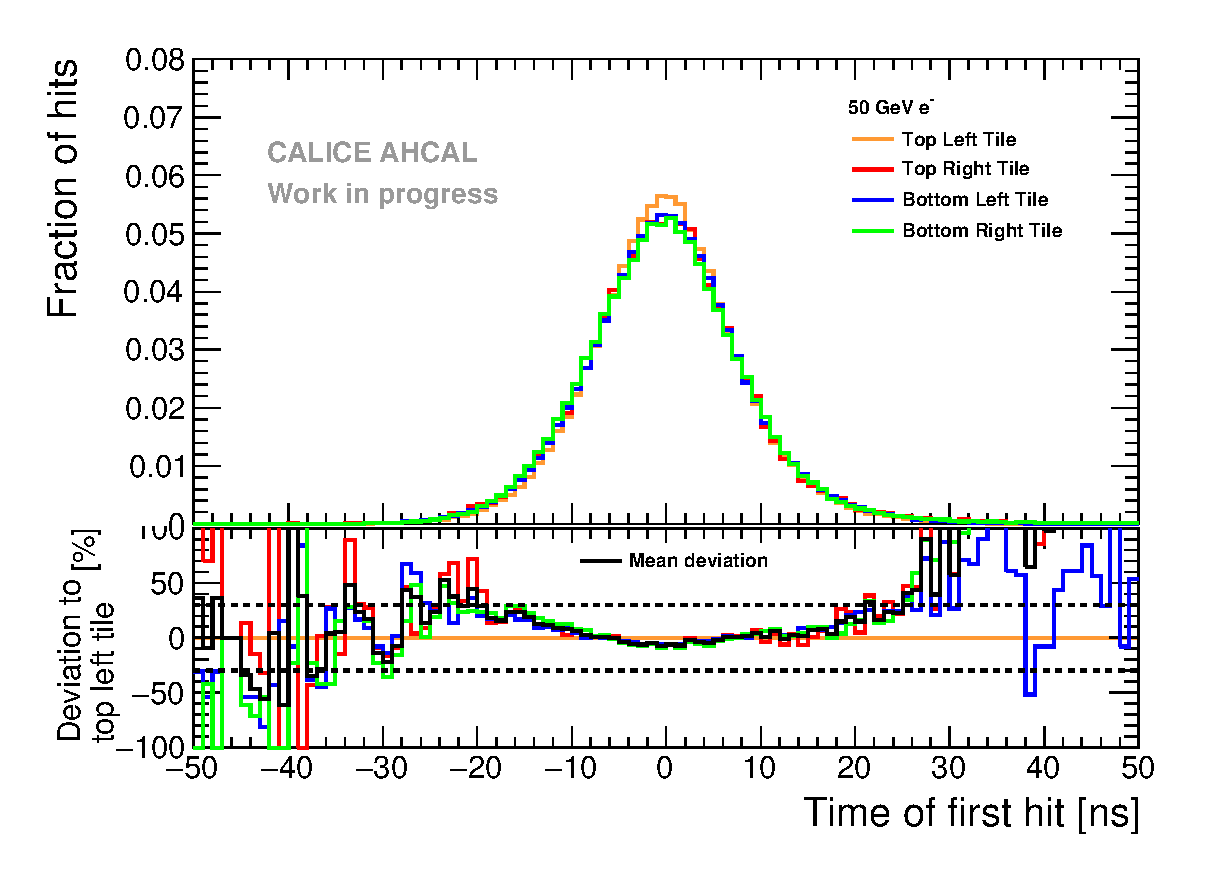
\includegraphics[width=1\textwidth]{../Thesis_Plots/Timing/Electrons/Plots/Systematic_Inhomogeneity_50GeV.eps}
		\caption{}\label{fig:timing_syst_50GeV}
	\end{subfigure}
	\caption{Time of the first hit distribution for events where the center of gravity of the shower is in the four center tiles for 10 GeV electrons on the left and 50 GeV electrons on the right. Under each figure, the deviation of each time distribution to the top left tile is shown. The mean deviation of the time distributions is shown in a black line. The dashed black line represents a 30\% deviation relative to the top left tile time distribution.} \label{fig:SystTimeElectrons}
\end{figure}

\section{Systematic uncertainties}

For a significant assessment of differences observed between data and simulations, systematic uncertainties must be evaluated. Several possible sources were identified:

\begin{itemize}
	\item Non-Linearity correction: A non-linearity correction (see section \ref{subsec:lin_corr}) is determined from data with a limited accuracy lead to a systematic uncertainty. The residuals of the correction give a systematic uncertainty at the level of 0.2 ns.
	\item Time walk correction: Similarly to the non-linearity correction of the data, the systematic uncertainty obtained from the residuals of the time walk correction (see section \ref{subsec:timewalk}) is in the order of 0.2 ns.
	\item Number of triggered channels correction: The correction for the number of triggered channels over 0.5 MIP in a chip results in a residual on the mean time of the first hit (see section \ref{subsec:ped_shift}). The systematic uncertainty varies between 2 to 3.9 ns. For the time of first hit distribution, a systematic uncertainty is applied bin-by-bin for electrons and pions in the region of -30 ns to 30 ns. Outside of this region, a systematic uncertainty of 50\% is taken (see section \ref{subsec:Systematic_Correction}). This systematic error is the most dominant over all other uncertainties.
	\item AHCAL energy scale: The energy scale of the AHCAL was determined using the muon dataset (see chapter \ref{chap:ECalibAHCAL}). A systematic uncertainty on the MIP scale of around 3.6\% was derived by dividing the muon sample in odd and even run numbers and by looking at the average spread of the fitted MIP value for both subsamples. This is converted to an uncertainty in time using the mean time of first hit as a function of the hit energy using the QGSP\_BERT\_HP physics list. At 0.5 MIP, this results in an uncertainty of 0.1 ns. For hits above 1 MIP, the uncertainty is below 0.05 ns.
	\item Global time smearing parameters: A global time smearing parametrization is used from muon data to smear the time in simulation. A bin-by-bin systematic uncertainty is applied to the time of first hit distribution to take into account the difference with a layer-wise time smearing parametrization.
	\item Number of triggered channels in a chip parametrization: A smearing parametrization of the width of the time distribution as a function of the number of triggered channels in a chip is obtained from the electron dataset. An error band on the width was obtained by comparing all electron energies (see appendix \ref{appendix:ped_shift}). This is applied to simulation for the systematics uncertainty on the width of the time distribution.
	\item Determination of the offset to $t=0$: For simulation, the time shift per layer is calculated using a time of flight correction $T_{of} = \frac{z_{layer}}{c}$ with $c$ the speed of light and $z_{layer}$ the z position of a layer. For this, an uncertainty of 3 mm corresponding to the scintillator thickness is taken in z corresponding to 0.01 ns uncertainty in timing.
	\item Cross-talk: No measurement for optical cross-talk between tiles is available and from previous measurements with the AHCAL physics prototype, it varies between 10\% and 18\% \cite{Gunter:2015ika}. The cross-talk value induces a different number of hits in the detector thus has an impact on the width of the time of first hit distribution. The variation of this parameter in the simulation for the layers 4 to 10 is used for systematics.
	\item Absolute number of events: In the pion data, some possible contamination from multi-particle events (mainly muons) may be present still after the selection. Thus, the number of true pion events is not known. The cluster time rejection method (see section \ref{sec:pionsel}) rejects up to 1\% of multi-particle events in the data. A conservative uncertainty of 10\% on the data normalization is assigned to each bin when comparing data to simulation for the absolute time of first hit distribution.
\end{itemize}

The systematic uncertainties are added in quadrature for the full systematic uncertainty assuming no correlation between uncertainties. For the mean time of the first hit as a function of the hit energy and as a function of the hit distance to the shower center of gravity, the systematic uncertainty is resulting at 0.3 ns for muons and between 2 to 4 ns for electrons and pions. The table \ref{table:time_syst} sums up the systematic uncertainties used in the analysis.

\begin{table}[htb!]
	\centering
	\caption{Summary of systematic uncertainties.}
	\label{table:time_syst}
	\begin{tabular}{@{} lc @{}}
		\toprule
		\multicolumn{1}{c}{Uncertainty source} & Full uncertainty \\
		\midrule
		Non-linearity correction & 0.2 ns (data)\\
		Time-walk correction & 0.2 ns (data)\\
		Number of triggered channels correction & 2 - 3.9 ns / bin-wise (e/$\pi$) (data)\\
		Energy Scale & 0.05-0.1 ns (data)\\
		Time of flight offset & 0.01 ns (MC) \\
		Cross-talk parameter & 10-18\% (MC)\\
		Global time smearing parameters & bin-wise (MC)\\
		Number of triggered channels in a chip parametrization & bin-wise (MC)\\
		Multi-particle events & 10\% ($\pi$) (data)\\
		\midrule
		\midrule
		\multicolumn{2}{c}{Resulting systematic uncertainties per distribution (data)} \\
		\midrule
		data-MC ToFH distribution & bin-wise (e) - bin-wise + 10\% ($\pi$) \\
		data-MC vs hit energy & 0.3 ns ($\mu$) - 1.8 to 3 ns (e/$\pi$)\\
		data-MC vs hit distance to shower CoG & 0.3 ns ($\mu$) - 1.8 to 3 ns (e/$\pi$)\\
		data-MC vs hit depth & 0.3 ns ($\mu$) - 1.8 to 3 ns (e/$\pi$)\\
		\bottomrule
	\end{tabular}
\end{table}

\section{Validation of the simulation}

The simulation is validated by comparing the recorded muon and electron data to simulations. The timing resolution is extracted from muon data runs by fitting a double Gaussian to the data in the range [-50 ns, 50 ns] and is used to smear the timing of simulated calorimeter hits. For the sake of simplifying the time smearing in the simulation, a global smearing parametrization is done. The table \ref{table:time_res_sim} summarizes up the parameters used.

\begin{table}[htb!]
	\centering
	\caption{Timing resolution extracted with a double Gaussian fit from muon data used for simulation.}
	\label{table:time_res_sim}
	\begin{tabular}{@{} cccccc @{}}
		\toprule
		$\alpha_{1}$ & $\mu_{1}$ [ns] & $\sigma_{1}$ [ns] & $\alpha_{2}$ & $\mu_{2}$ [ns] & $\sigma_{2}$ [ns] \\
		\midrule
		0.607352 & -0.699095 & 5.85891 & 0.391041 & 0.945274 & 3.4012 \\
		\bottomrule
	\end{tabular}
\end{table}

The comparison of the time of first hit distribution for muons between data and simulations is shown in figure \ref{fig:sim_data_muon}. The comparison shows that in the range of -20 ns to 20 ns, data and simulation agree well within the uncertainties. In this range, the smearing with a double Gaussian in the simulation reproduces well the data. However, outside this range, the simulation underestimates the tails. This is probably caused by the noise implementation in simulation that does not perfectly reproduce the data. The time of distribution has been checked layer-by-layer and compared to simulations. Similar, the agreement between data and simulations is best in the range of -20 ns to 20 ns and the tails are not perfectly reproduced in simulation.

\begin{figure}[htbp!]
	\centering
	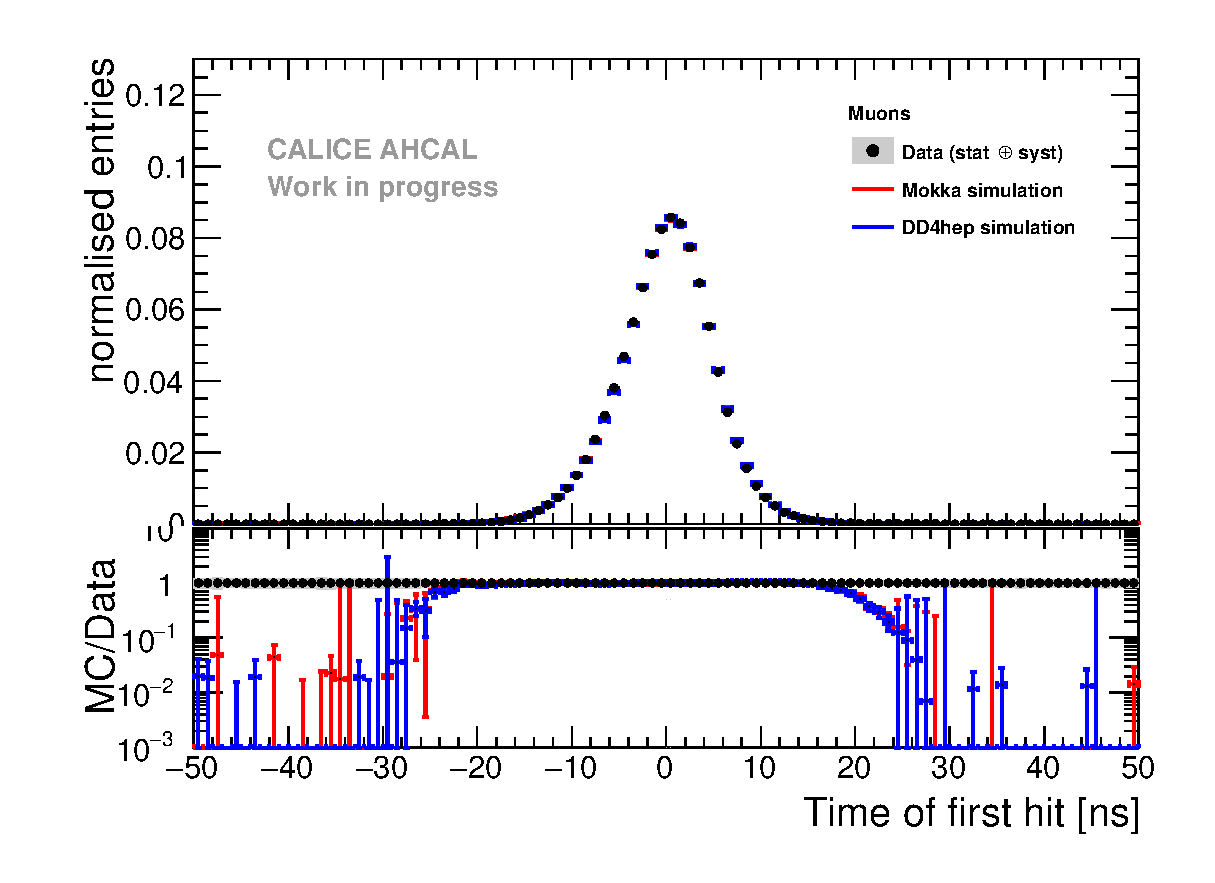
\includegraphics[width=0.6\textwidth]{../Thesis_Plots/Timing/Muons/Plots/Comparison_MokkaDD4hepData_Muons.eps}
	\caption{Time of first hit distribution for muons in data and simulation between -50 and 50 ns. The grey area represents the statistical uncertainty of the data. The error bars of the simulation are obtained by varying the cross-talk parameter between 10\% and 18\% and taking into account the error of a global time smearing parametrization.}
	\label{fig:sim_data_muon}
\end{figure}

\begin{figure}[htbp!]
	\centering
	\begin{subfigure}[t]{0.49\textwidth}
		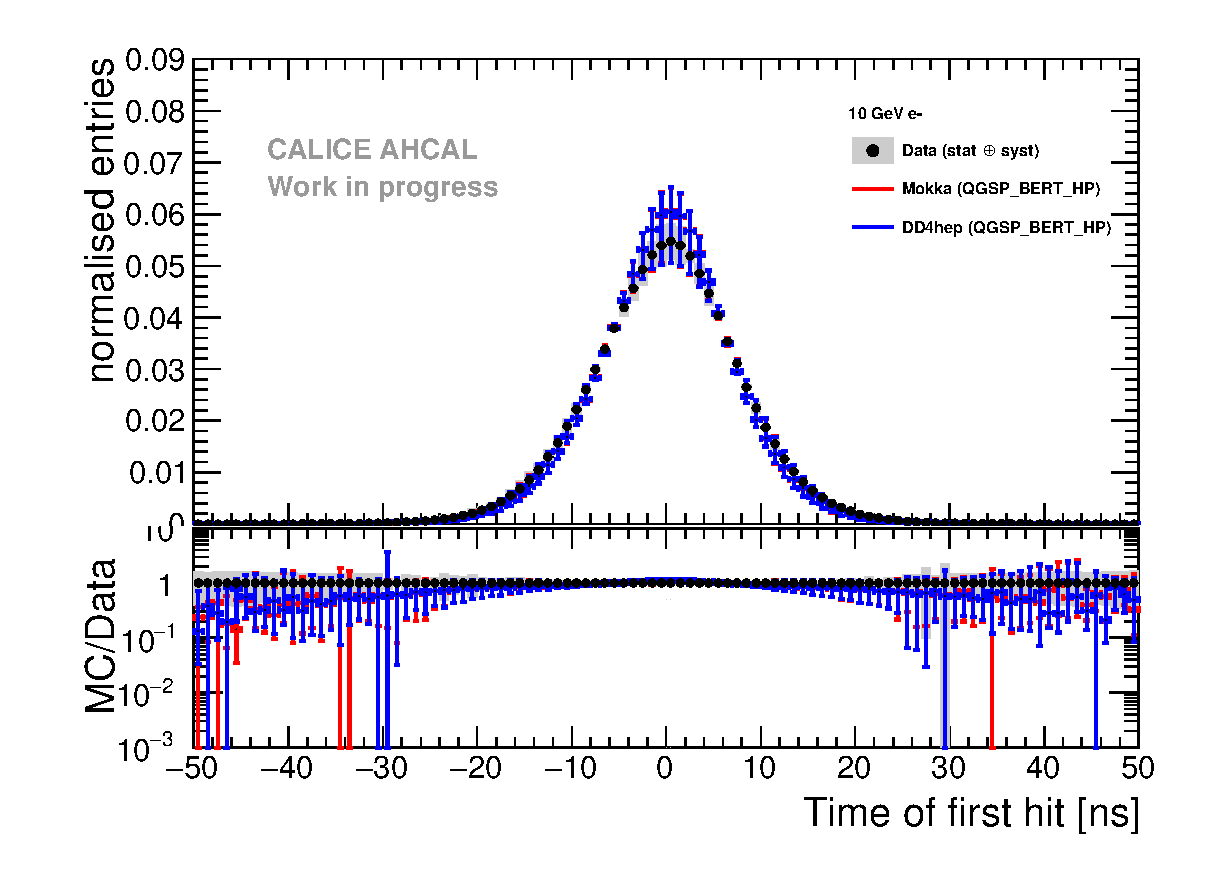
\includegraphics[width=1\textwidth]{../Thesis_Plots/Timing/Electrons/Plots/Comparison_SimData_Electrons10GeV.eps}
		\caption{}\label{fig:elec_sim_data_10GeV}
	\end{subfigure}
	\hfill
	\begin{subfigure}[t]{0.49\textwidth}
		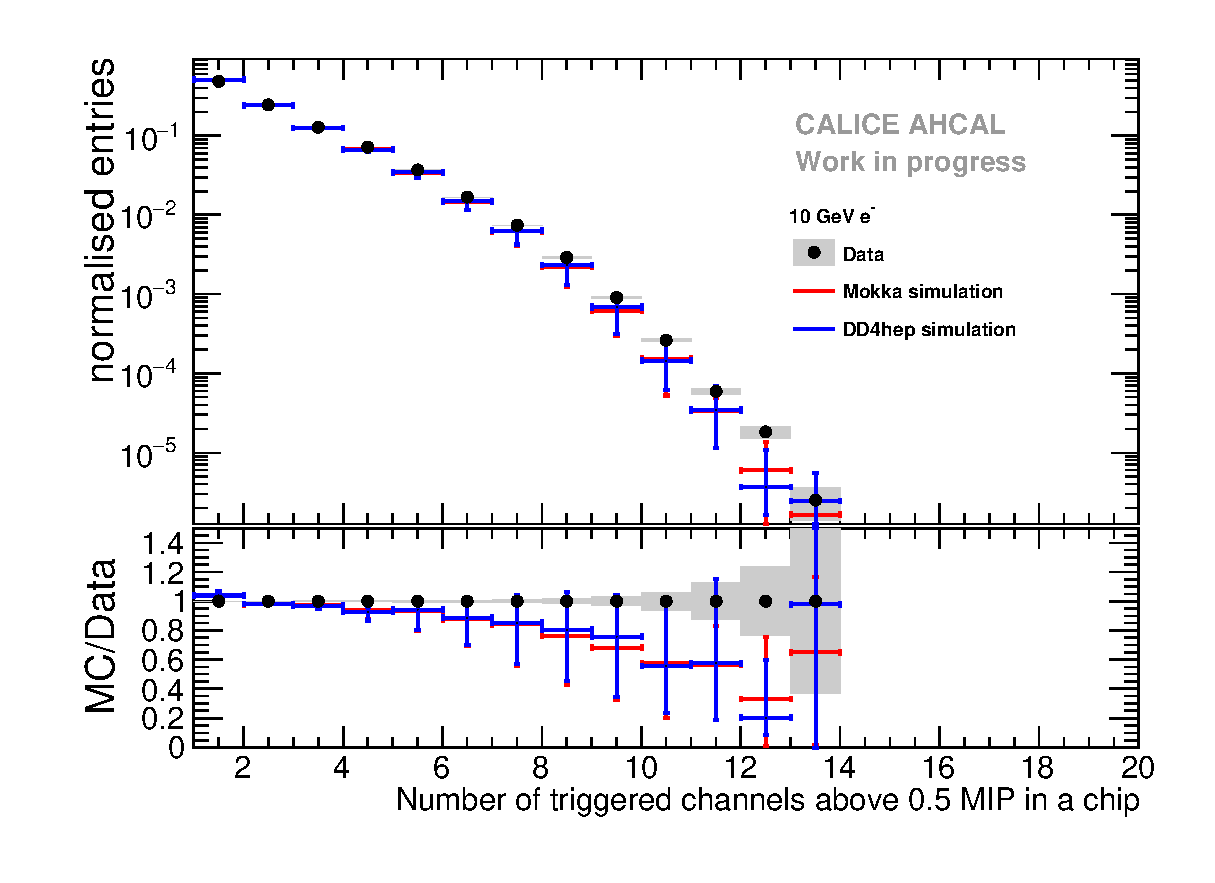
\includegraphics[width=1\textwidth]{../Thesis_Plots/Timing/Electrons/Plots/Comparison_SimData_Electrons_nHits_10GeV.eps}
		\caption{}\label{fig:elec_sim_data_nHits_10GeV}
	\end{subfigure}
	\caption{\subref{fig:elec_sim_data_10GeV}) Comparison of the time of first hit between data and simulations for 10 GeV electrons. The grey area represents the statistical and systematical error of the data. Error bars in simulation are obtained by varying the cross-talk parameter between 10\% and 18\% and with the uncertainty on parametrization of the width of the time distribution as a function of the number of triggered channels in a chip. \subref{fig:elec_sim_data_nHits_10GeV}) Comparison of the number of triggered channels per chip between data and MC for 10 GeV electrons. The grey area represents the statistical error of the data. Error bars in simulation are obtained by varying the cross-talk parameter between 10\% and 18\%.}
\end{figure}

To further validate the simulation, a comparison with electron data has been done. In addition to the muon resolution, a parametrization of the increase of the width of the time distribution as a function of the number of triggered channels in a chip above 0.5 MIPs is added in simulation (see appendix \ref{appendix:ped_shift}). The figure \ref{fig:elec_sim_data_10GeV} shows the comparison of the time of first hit distribution for 10 GeV electrons in data and simulation. The errors bars in the simulation are obtained by varying the cross-talk parameter between 10\% and 18\%, taking into account the global time smearing parametrization uncertainty and from the uncertainty of the parametrization of the increase of the width of the time distribution as a function of the number of triggered channels in a chip. The last uncertainty is dominant over the other uncertainties.

The simulation is systematically narrower than data. This is caused by the simulation having fewer hits in a chip than data which can be seen in figure \ref{fig:elec_sim_data_nHits_10GeV}. The simulation is generally 10\% to 20\% lower than data in the region of 6 to 10 hits per chip. Overall, the simulation describes well the data within statistical and systematic uncertainties in the central region of -30 ns to 30 ns for all energies. The error bars in the simulation is due to the parametrization of the increase of the width. However, the description of the tails of the time of first hit distribution in the simulation are well underestimated. As for muons, this is probably due to the description of the noise in the simulation that does not perfectly reproduce the data. The time of first hit distributions and the distribution of the number of triggered channels per chip have been checked for all energies and they can be seen in appendix \ref{appendix:TimingAdd}.

\begin{center}
	\rule{0.5\textwidth}{.4pt}
\end{center}

In this chapter, the timing analysis of the recorded electron data has been presented. A time resolution (RMS) for the AHCAL in electron beams is obtained between 7.8 ns at 10 GeV beam energy and 8.5 ns at 50 GeV beam energy. An increase of the width of the time distribution as a function of the number of triggered channels in a chip is observed in the electron data. This electronic effect has been parametrized and it is used as an input to tune the simulation in order to reflect the data.

The AHCAL timing simulation has been validated by comparing the simulated time distributions to data using muons and electrons. Overall, the simulation reproduces the data within 20\% in the range of -30 ns to 30 ns. In addition, the simulation underestimates highly the tails of the distribution that is due to an imperfect implementation of noise hits in the simulation.

However, the simulation is in good enough agreement with data that the time of hadron showers can be studied. In the next chapter, the timing analysis of pion showers and comparisons to simulation will be presented.
